% !TEX TS-program = lualatex
% !BIB TS-program = biber
%\documentclass[handout]{beamer}
\documentclass{beamer}
\input{../common/misomva}
%\newcommand{\misoclasstinytitleslide}{Partially based on material by:  Ulrike von Luxburg, \\[-1em] Gary Miller, Doyle \& Schnell, Daniel Spielman}
\newcommand{\misoclasstinytitleslide}{Partially based on material by:   Gary Miller, \\ Mikhail Belkin, Branislav Kveton, \\[-1em] Doyle \& Schnell, Daniel Spielman}
\newcommand{\misoclassdate}{}
\begin{document}
% Topic-specific title slide
\newcommand{\topictitle}{SSL Manifold Regularization}
\newcommand{\topicsubtitle}{Manifold Regularization and Laplacian SVMs}
\renewcommand{\misoclasstinytitleslide}{Partially based on material by:  Mikhail Belkin, Partha Niyogi, \\[-1em] Olivier Chapelle, Bernhard Sch\"olkopf}

\MakeTopicSlide

\begin{frame}
\frametitle{SSL with Graphs: Manifold Regularization}
General (S)SL objective:
\[
 \min_{f}  \sum_i^{n_l} \mcolA{V(\bx_i, y_i, f\left( \bx_i \right))} + \lambda 
\mcolB{\Omega(f)}
\]

Want to control $f$, also for the out-of-sample data, i.e.,\@ \emphcol{everywhere}. \pause
\[
\mcolB{\Omega(f)} = \lambda_2\bff\transpose\bL\bff +  \lambda_1\pause \int_{\bx \in \cX} f(\bx)^2 \diff \bx  
\]
\pause
For general \emphcol{kernels}:

\[
 \min_{f \in \cH_\cK}  \sum_i^{n_l} \mcolA{V(\bx_i, y_i, f\left( \bx_i \right))} 
+ \lambda_1 \mcolB{ \|f\|^2_\cK }
+ \lambda_2 \mcolB{ \bff\transpose\bL\bff }
\]

\end{frame}
%%%%%%%%%%%%%%%%%%%%%%%%%%%%%%%%%%%%%%%%%%%%%%%%%%%%%%%%%%%%
\begin{frame}
\frametitle{SSL with Graphs: Manifold Regularization}

\[
f^\star = \argmin_{f \in \cH_\cK}  \sum_i^{n_l} \mcolA{V\left(\bx_i, y_i, f\right)} 
+ \lambda_1 \mcolB{ \|f\|^2_\cK }
+ \lambda_2 \mcolB{ \bff\transpose\bL\bff }
\]
\pause
\begin{block}{Representer theorem for manifold regularization}
\pause The minimizer $f^\star$ has a \textbf{finite} expansion of the form \pause
\[
f^\star(\bx) = \sum_{i=1}^{n_l + n_u} \alpha_i \cK(\bx,\bx_i)
\] 
\end{block}
\pause
 
$\mcolA{V\left(\bx, y, f\right)} = \pause \left( y - f\left( \bx \right)\right)^2$
\\  
\pause
\begin{flushright}
\emphcol{LapRLS} Laplacian Regularized Least Squares\end{flushright}
\pause
$\mcolA{V\left(\bx, y, f\right)} = \pause  \max\left(0,1-yf\left(\bx\right)\right)$
\\
\pause
\begin{flushright}
\emphcol{LapSVM} Laplacian Support Vector Machines\end{flushright}
\end{frame}
%%%%%%%%%%%%%%%%%%%%%%%%%%%%%%%%%%%%%%%%%%%%%%%%%%%%%%%%%%%%
\begin{frame}
\frametitle{SSL with Graphs: Laplacian SVMs}
\[
f^\star = \argmin_{f \in \cH_\cK}  \sum_i^{n_l} \mcolA{\max\left(0,1-yf\left(\bx\right)\right)} 
+ \gamma_A \mcolB{\|f\|^2_\cK }
+ \gamma_I \mcolB{ \bff\transpose\bL\bff }
\]
\pause
Allows us to learn a function in \emphcol{RKHS}, i.e., 
\emphcol{RBF} kernels.
\pause
\begin{center}
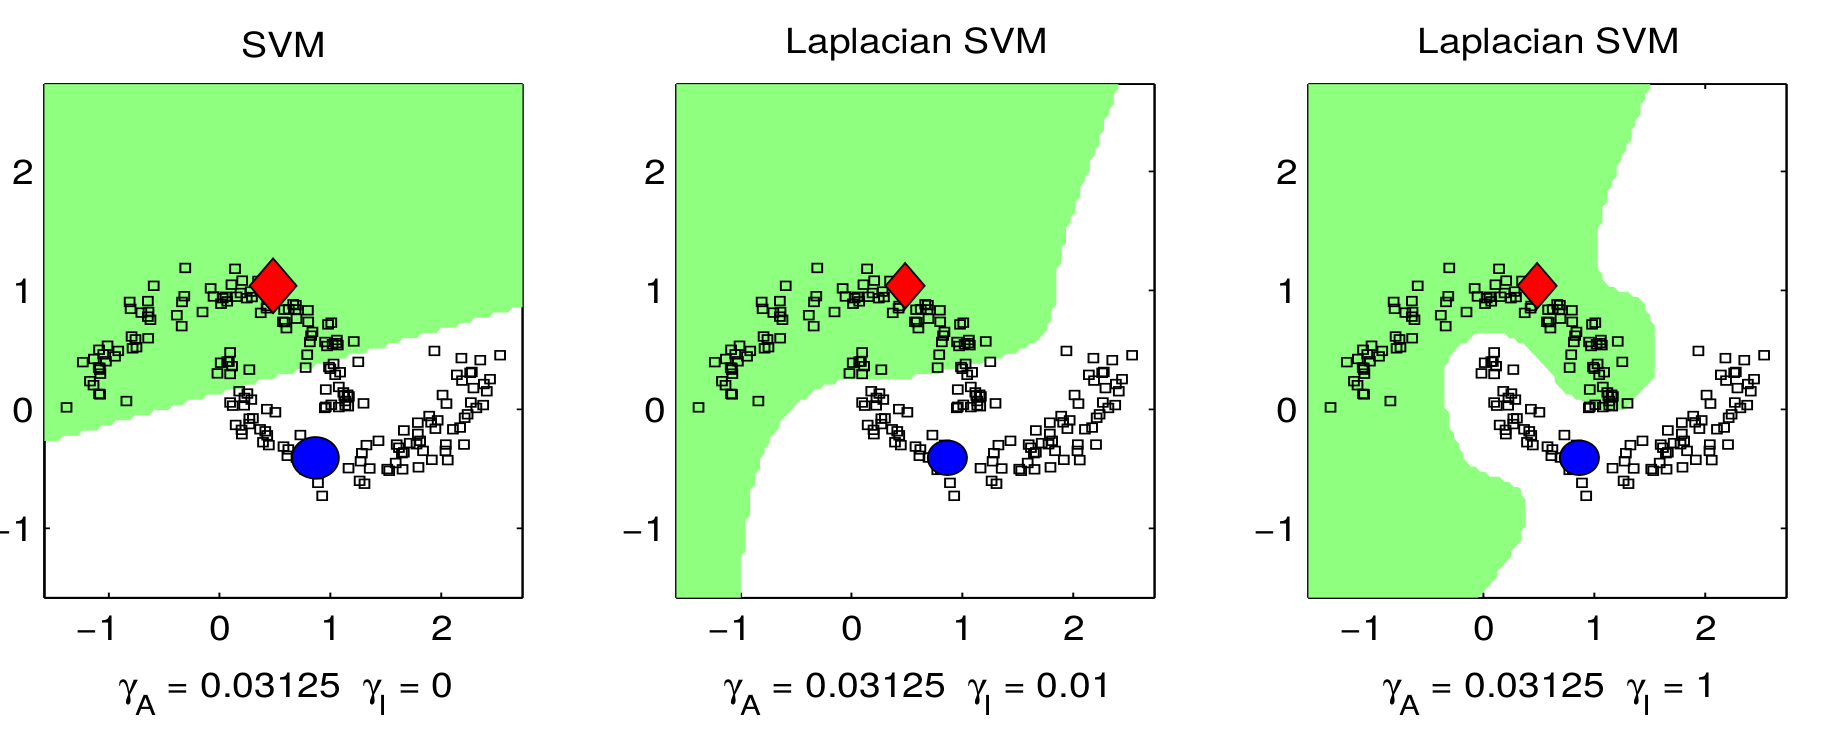
\includegraphics[width=\columnwidth]{../img/lapsvmrbf}
\\[0.5em] {\tiny Source: \citet{belkin2006manifold}}
\end{center}
\end{frame}
%%%%%%%%%%%%%%%%%%%%%%%%%%%%%%%%%%%%%%%%%%%%%%%%%%%%%%%%%%%%
\begin{frame}
\frametitle{SSL with Graphs: Laplacian SVMs}
\begin{center}
%
\includegraphics[width=0.8\columnwidth]{img/lapsvmrbf}\\
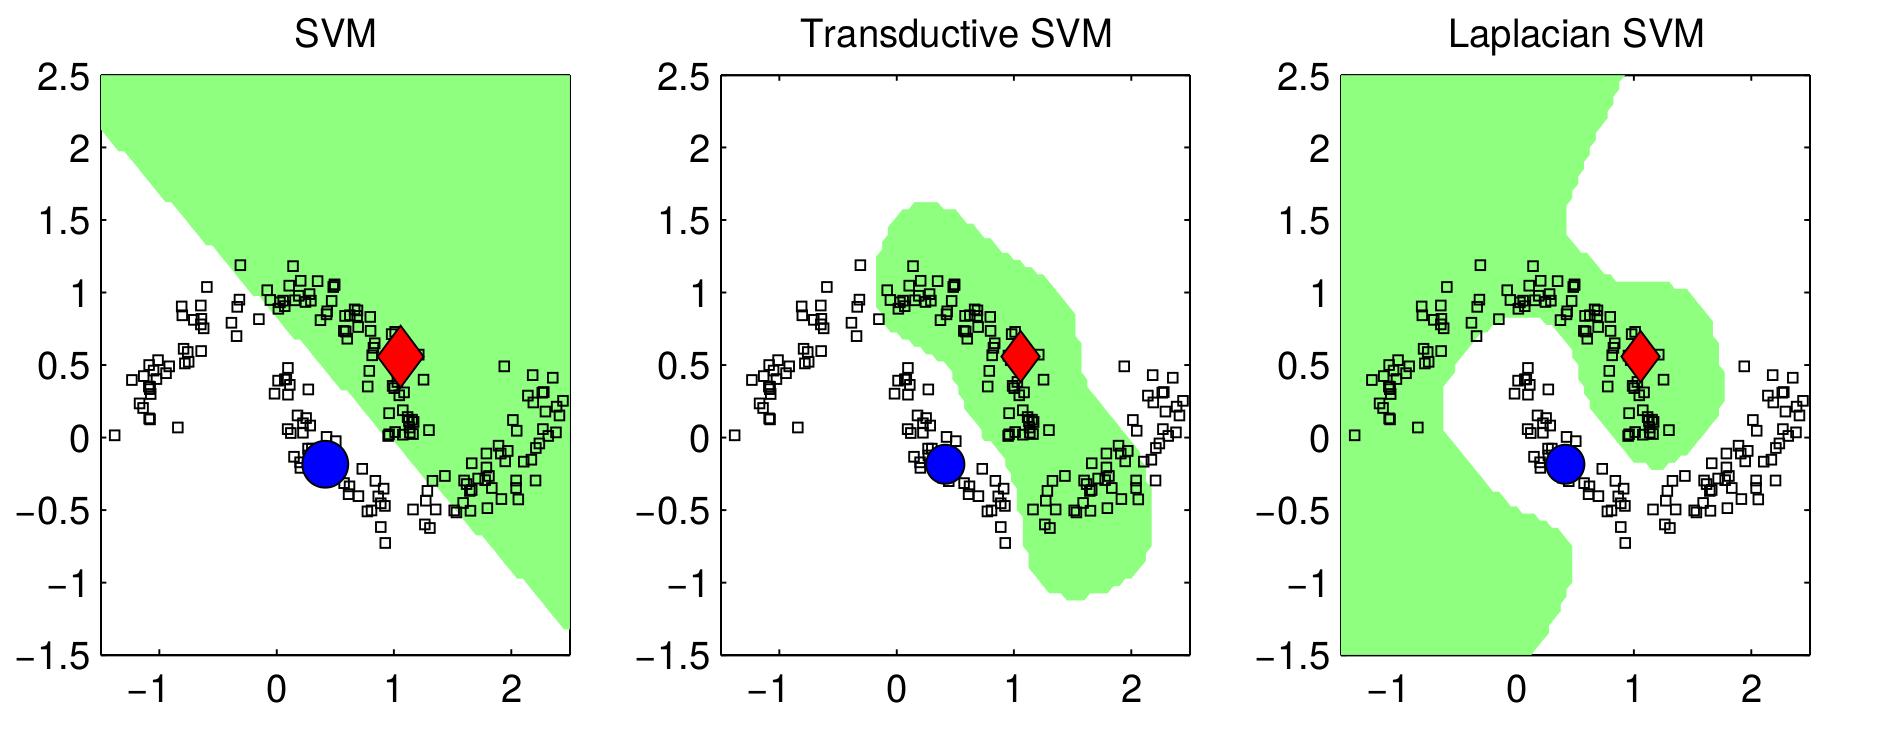
\includegraphics[width=0.84\columnwidth]{../img/lapsvmrbf2}
\\[0.5em] {\tiny Source: \citet{belkin2006manifold}}
\end{center}
\end{frame}
%%%%%%%%%%%%%%%%%%%%%%%%%%%%%%%%%%%%%%%%%%%%%%%%%%%%%%%%%%%%



\begin{frame}
%\frametitle{Where we left off}
\frametitle{Checkpoint 1}

Semi-supervised learning with graphs:
  \[
   \min_{\bff  \in \{\pm 1\}^{n_l + n_u} }\mcolA{(\infty) \sum_{i=1}^{n_l} w_{ij} \left( f(\bx_i) - y_i \right)^2}
   + \lambda\mcolB{\sum_{i,j=1}^{n_l+n_u} \left( f(\bx_i)  - f(\bx_j)  \right)^2}
  \]
  
  \vspace{2em} \pause
  
Regularized harmonic Solution:
\[
 \bff_{u} = \left( \bL_{uu} + \alert{\gamma_g \bI} \right)^{-1}(\bW_{ul}\bff_{l})
\]


\end{frame}

%%%%%%%%%%%%%%%%%%%%%%%%%%%%%%%%%%%%%%%%%%%%%%%%%%%%%%%%%%%%

\begin{frame}
\frametitle{Checkpoint 2}
%\frametitle{Where we left off}

Unconstrained regularization in general:

\begin{equation*}
  \bff^{\star} = \min_{\bff \in \R^\nodes}  \mcolA{(\bff - \by)\transpose \bC (\bff - \by)} + \mcolB{\bff\transpose \bQ \bff}
\end{equation*}

\vspace{2em} \pause

Out of sample extension: Laplacian SVMs

\[
f^\star = \argmin_{f \in \cH_\cK}  \sum_i^{n_l} \mcolA{\max\left(0,1-yf\left(\bx\right)\right)} 
+ \lambda_1 \mcolB{ \|f\|^2_\cK }
+ \lambda_2 \mcolB{ \bff\transpose\bL\bff }
\]

\end{frame}



\MakeLastSlide
\end{document}
